\documentclass[../main.tex]{subfiles}

\begin{document}
	 \section{Die marktwirtschaftliche Legalisierung}
	 
	 \subsection{Definition}
	 Die marktwirtschaftliche Legalisierung ist eine Art der Legalisierung, bei der der Markt so wenig wie möglich eingeschränkt wird, so dass die Allokation der Ressourcen über den Marktpreis koordiniert wird.
	 Eine Marktwirtschaft ohne staatliche Regulierungen reguliert sich selbst und stellt sich beim ökonomischen Marktgleichgewicht ein.
	 
	 
	 \subsection{Ein mögliches Schweizer Modell}
	 Die in der Arbeit angesprochene Legalisierung soll den Anspruch der Verdrängung des Schwarzmarktes so weit wie möglich erfüllen.
	 Der marktwirtschaftliche Ansatz Kanadas eignet sich für die Erfüllung dieses Zieles.
	 Ein Nebenziel, gefährdete Gesellschaftsgruppen zu schützen, wird durch eine Legalisierung weiterhin gestärkt, da der Jugendschutz erst auf den legalen Markt einwirken kann.
	 Das potentielle Schweizer Konzept ist so aufgebaut, dass sowohl Konsum und Besitz als auch Handel und Anbau unter bestimmten Bedingungen legal ist.
	 Niemand soll am Markteintritt gehindert werden, solange er sich an die Rahmenbedingungen hält.\\
	 
	 \noindent
	 Ausser den unten genannten Einschränkungen soll die Ressourcenallokation dem freien Markt überlassen werden. 	 
	 Massnahmen zur Minderung der Prävalenzen gehen über die Nachfrageseite und nicht wie bei der Repression über die Angebotsseite.
	 Die Auswirkungen des Eingreifens werden im Kapitel \texttt{Die marktwirtschaftliche Legalisierung > Ökonomie > Preis} genauer erklärt.
	 
	 
	 \subsection{Ökonomie}
	 
	 \paragraph{Preis}
	 Bei einer marktwirtschaftlichen Legalisierung würde der Marktpreis sofort fallen, da sich der Preis beim Marktgleichgewicht eingliedern würde. 
	 Der Marktpreis würde sich dem Einstandspreis anpassen und die Ressourcenallokation wäre über den Markt gesteuert.
	 Dass sich der Preis nach einer Legalisierung immer weiter senken würde, konnte man auch in Colorado beobachten.
	 (Siehe Abbildung \ref{fig:equilibrium})
	 
	 \noindent	 
	 \begin{figure}[H]
	 	\centering
		\includegraphics[height=7cm]{example-image-a}
		\captionsetup{font=small}
		\caption[Preis-Mengen-Diagramm ohne Massnahmen]{Preis-Mengen-Diagramm ohne Massnahmen\protect\footnotemark}		
		\label{fig:equilibrium}
	 \end{figure}
	 \footnotetext{\cite{TODO}}
	 
	 
	 Im Gegensatz zu den repressiven Massnahmen setzt die Fokussierung auf präventive Massnahmen nicht an der Anbieterseite, sondern an der Nachfrageseite an.
	 (Siehe Abbildung \ref{fig:prevention})
	 \noindent	 
	 \begin{figure}[H]
	 	\centering
		\includegraphics[height=7cm]{example-image-a}
		\captionsetup{font=small}
		\caption[Preis-Mengen-Diagramm mit präventiven Massnahmen]{Preis-Mengen-Diagramm mit präventiven Massnahmen\protect\footnotemark}		
		\label{fig:prevention}
	 \end{figure}
	 \footnotetext{\cite{TODO}}
	 
	 
	 % Minimum und Maximum
	 
	
	 
	 
	 
	 \subsection{Rechtslage \& Einschränkungen}
	 
	 \subsubsection{Cannabisgesetz}
	 Die Legalisierung kann nicht ohne Einschränkungen erfolgen und deswegen muss man ein neues Gesetz in Betracht ziehen.
	 Als Beispiel dienen Gesetze über den Umgang mit Tabak und Alkohol.
	 Der gesetzliche Umgang mit Alkohol und mit Tabak, zwei legalen psychoaktiven Substanzen wird in eigenen Gesetzen geregelt. 
	 Aus diesem Grund müsste man für Cannabis ein neues Gesetz mit Verordnungen erlassen, das die Herstellung, Einfuhr und Ausfuhr, Verkauf und Besteuerung regeln würde.	 
	 Im Cannabisgesetz werden alle in den folgenden Untersektionen genannten Einschränkungen weiter konkretisiert.
	 
	 \subsubsection{Besteuerung}
	 Eine Cannabissteuer muss schon auf der höchsten Stufe der Normenhierarchie geregelt werden. 
	 Die Rechtsgrundlage der Besteuerung wird der von Alkohol und Tabak gleichen, da es sich bei allen drei Produkten um psychoaktive Substanzen handelt.
	 Die besondere Verbrauchssteuer nach \texttt{Art. 131 Abs. 1 BV} muss so erweitert werden, dass der Bund diese auch auf Cannabis und dessen Produkte erheben kann.
	 Die Einnahmen der Verbrauchssteuern sollen in Prävention und Behandlung von Suchtproblemen aber auch in die vorhandenen Ausgleichskassen fliessen.
	 Mit der Erweiterung von \texttt{Art. 131 Abs. 3 BV} für Prävention und Therapie und \texttt{Art. 112 Abs. 5 BV} für die AHV und IV mit Cannabis, ist die Grundlage für eine Besteuerung geebnet.\\
	 
	 \noindent
	 Nähere Bestimmungen über die Besteuerung würden im neuen Cannabisgesetz festgelegt werden.
	 Es existieren viele Faktoren, die sich für eine Besteuerungsgrundlage eignen würden, jedoch bewies sich die Besteuerung nach absolutem Inhalt bereits zahlreich.
	 Tabak- und Alkoholprodukte werden nach gleichem Prinzip besteuert und tragen einen wesentlichen Teil der Deckung der Schäden bei.
	 Auch Ausgleichskassen wie die AHV oder IV werden durch die Steuerlast der Produkte teilfinanziert.
	 Eine Besteuerung nach absolutem THC Gehalt ist der gewichtsbasierten Besteuerung zu bevorzugen, da sich dann keine Anreize für die Hersteller ergeben, den THC Gehalt künstlich hochzuzüchten.
	 Eine höhere Besteuerung auf potenteres Cannabis sollte chronische Konsumenten abhalten, immer potenteres Cannabis zu konsumieren, das einen höheren Schaden verursacht. \\
	 
	 \noindent
	 Das Ausmass der gesamten Besteuerung wird im Kapitel \texttt{Legalisierung > Besteuerung} ermittelt.
	 Das Ziel der marktwirtschaftlichen Legalisierung ist es, die Allokation der Güter möglichst dem Markt zu überlassen.
	 Um das Steueraufkommen quantitativ zu berechnen, wird ein Maximum und Minimum ermittelt, wovon man das Minimum anstreben sollte.
	 
	 
	 
	 \subsubsection{Jugendschutz}
	 In erster Linie dient der Jugendschutz dem Wohle der Kinder und Jugendliche, dass sie von den Risiken des Betäubungsmittelkonsums geschützt werden und ihre psychische und physische Entwicklung nicht beeinträchtigt wird. 
	 Eine bereits existierende Einschränkung im Jugendschutz stellt das Abgabealter von Alkohol an Jugendliche dar, das sich bei 18 Jahren befindet (\texttt{Art. 41 Abs. 1 lit. i AlkG}). 
	 Bei Cannabis würde man auch ein Schutzalter zwischen 18 - 20 Jahren anstreben. 
	 Dies ist sinnvoll, da die Gehirnentwicklung des Menschen sich ab dem 18. Lebensjahr verlangsamt und bei ungefähr 25 Jahren weitgehend abgeschlossen ist.\footcite{arain-2013}
	 Zwar ist die Gehirnentwicklung bei einem 18-jährigen Erwachsenen noch nicht vollständig abgeschlossen, jedoch kann man annehmen, dass eine Person ab diesem Alter mehr Eigenverantwortung übernehmen kann.
	 Es wäre kontraproduktiv, einem Teil der grössten Gruppe an Konsumenten den Zugang zum legalen Markt zu verweigern, da diese sonst auf den Schwarzmarkt ausweichen.\\
	 
	 \noindent
	 Der Kern des Jugendschutzes besteht zwar primär aus einem Abgabeverbot an Jugendliche, jedoch müssen auch alle anderen Massnahmen der Vier-Säulen-Politik umgesetzt werden. 
	 Als direkte Auswirkung folgt, dass bereits konsumierende Jugendliche Hilfe bei der Bewältigung ihrer Sucht zur Verfügung gestellt bekommen. 
	 Neben der Suchthilfe für chronische Konsumenten ist auch die Früherkennung und Intervention von grosser Bedeutung. 
	 Durch eine Legalisierung wird der Konsum nicht mehr stark stigmatisiert, sodass Bezugspersonen die Situationen frühzeitig erkennen und handeln können. 
	 Die Prävention erhalten alle Jugendliche, sodass Kinder und Jugendliche wichtige Kompetenzen erlernen, sich gegen den Konsum von Betäubungsmitteln zu stellen.  
	 
	 \subsubsection{Werbeeinschränkungen}
	 Die Vier-Säulen-Politik der Schweizer Drogenpolitik gibt das Ziel vor, den Konsum von psychoaktiven Substanzen so weit wie möglich zu mindern.
	 Ein gutes Marketing bewirkt das Gegenteil, es führt zu einer Erhöhung der Absatzzahlen.
	 Den Unternehmen sind ohne Einschränkungen unzählige Möglichkeiten geboten, ihr Produkt so positiv wie möglich darzustellen.	 
	 Vor allem Jugendliche und junge Erwachsene können durch Werbung stark beeinflusst werden.
	 Als Beispiel dient dabei Werbung für Tabakprodukte und für Alkohol.
	 Viele Unternehmen in diesen Bereichen sind zwar der Meinung, dass ihre Werbung nicht jüngere Menschen beeinflussen würde, jedoch wurde dies in mehreren Studien widerlegt.
	 Sowohl Werbung für Tabak \footcite{lovato} als auch für Alkohol \footcite{jernigan} kann das Konsumverhalten beeinflussen.
	 Manche Werbungen vermitteln ein positives Gefühl und zeigen eine gewisse Normalität auf. 
	 So wird den Menschen nur positive Effekte vermittelt, während negative Effekte nicht erwähnt werden.
	 Da es sich bei allen Produkten um psychoaktive Substanzen handelt, kann man diese Beobachtungen auf Cannabisprodukte ableiten.
	 Das Ziel der Einschränkungen ist nicht, Werbung komplett zu verbieten, sondern sie so zu regulieren, dass sie keine falschen Informationen vermittelt.\\
	 
	 \noindent	 
	 Einschränkungen über die Werbung von Cannabis würden im Cannabisgesetz geregelt werden und würden dem Vorbild des Alkoholgesetzes, namentlich \texttt{Art. 42b AlkG}, folgen.
	 Der Kerngedanke der Einschränkungen besteht daraus, dass Nichtkonsumierende kein falsches Bild von den Produkten bekommen und nicht zum Konsum verleitet werden.
	 Der Begriff von Werbung beschränkt sich nicht nur auf digitale Werbung im Fernsehen oder auf Plakaten, sondern auch auf Wettbewerbe, Sponsorings und weiteren Kundenbindungsmassnahmen.
	 
	 	 
	 \subsubsection{Strassenverkehrsgesetz}
	 Unter aktueller Rechtslage herrscht ein komplettes Verbot von Cannabis im Strassenverkehr. 
	 Dies ist unteranderem dem zuzuschreiben, dass der Inhaltsstoff THC akut negative Effekte auf die kognitiven Fähigkeiten haben kann.	 
	 In der Verkehrsregelnverordnung nach \texttt{Art. 2 Abs. 2 VRV} führt schon der geringste Anteil an THC zur Fahrunfähigkeit.
	 Im Gegensatz zu Alkohol gilt für Cannabis die Nulltoleranz im Strassenverkehr.
	 Als Nachweis gilt schon die extrem geringe Menge von 1.5 µg/L nach \texttt{Art. 34 VSKV-ASTRA}.
	 Der Wert bleibt jedoch noch stundenlang über diesem Grenzwert, ohne dass der Konsument eine Wirkung spürt.
	 Bei regelmässigen Konsumenten existiert das Problem, dass das sich THC im Fettgewebe anreichern kann, sodass der Wert auch noch Tage danach über dem Grenzwert wäre. \\
	 
	 \noindent	 
	 In einer Studie wurde ermittelt, dass von Fahrern mit einer Konzentration von 8.2 µg/L im Blut ein ähnliches Unfallrisiko ausgeht wie von Fahrern mit einer Alkoholkonzentration von 0.5 Promille.\footcite{hartman-2015}
	 Man hat festgestellt, dass Fahrer, die Cannabis konsumiert haben, teilweise von der idealen Fahrbahn abwichen.
	 Fahrer mit THC Einfluss stellen aber im Gegensatz zu alkoholisierten Fahrern dennoch eine kleinere Gefahr dar, da sie keine erhöhte Bereitschaft zum Beschleunigen zeigen und die Fahrbahn nicht häufiger verlassen.
	 Die Gleichstellung der Blutkonzentration von THC und Alkohol bezieht sich somit nur auf das Halten der idealen Fahrbahn.\\
	 
	 
	 \noindent	 
	 \begin{figure}[H]
	 	\centering
		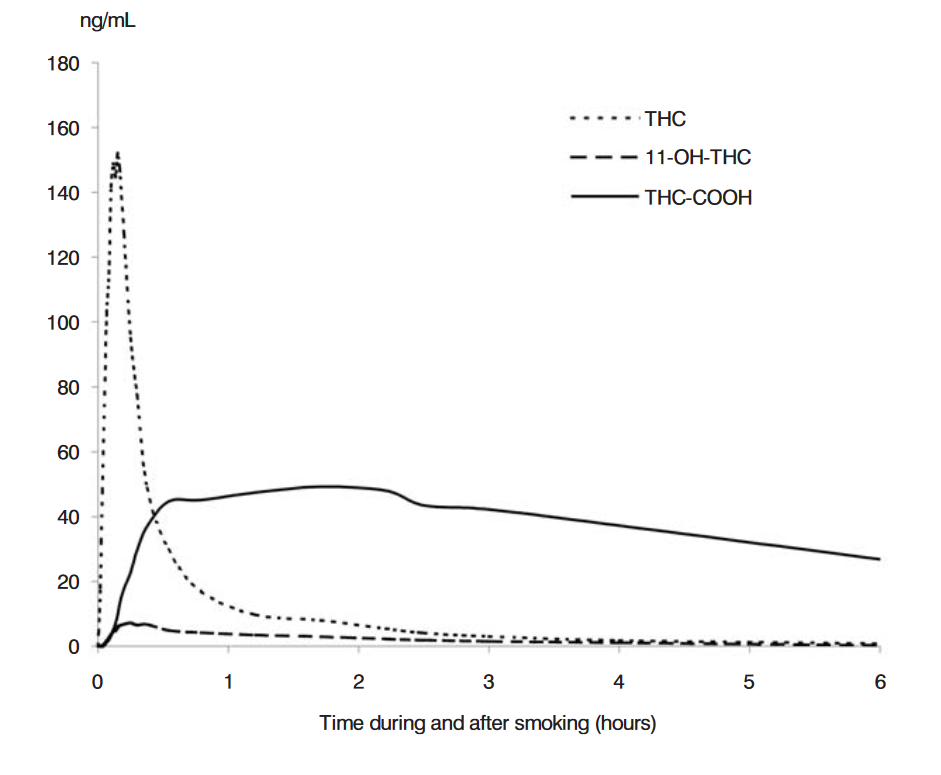
\includegraphics[height=10cm]{THCKonzentration}
		\captionsetup{font=small}
		\caption[Entwicklung der THC Konzentration im Blut]{Entwicklung der THC Konzentration im Blut\protect\footnotemark}		
	 \end{figure}
	 \footnotetext{\cite{giroud}}
	
	 
	 \noindent \\
	 Mit einer Legalisierung sollte ein Grenzwert in Betracht gezogen werden.
	 Der Grenzwert sollte sich am bereits bestehenden Alkoholgrenzwert von 0.5 Promille orientieren. 
	 Vor allem sinnvoll wäre dieser Grenzwert für regelmässige Konsumenten, bei denen der Wert nur langsam sinkt.
	 Mit der neuen Regelung wären regelmässige Konsumenten bereits nach mehreren Stunden rechtlich wieder fahrfähig.
	 
	 
	 \subsection{Besteuerung}
	 Durch die Legalisierung und neue Rechtslage besteht die Möglichkeit, dass Cannabis besteuert werden kann.
	 Der Staat kann mehr Einnahmen für die Staatskasse generieren und den Marktpreis direkt beeinflussen.
	 Erhöhte Steuern würden sich direkt im Marktpreis wiederspiegeln.
	 Die Besteuerung erfolgt auf verschiedenen Stufen und indirekte Steuern werden auch berücksichtigt.
	 
	 \paragraph{Mehrwertsteuer}
	 Die Mehrwertsteuer ist eine universelle Steuer und wird auf den Bruttoverkaufspreis erhoben.
	 Sie ist im Bundesgesetz über die Mehrwertsteuer (MWSTG) geregelt.
	 Nach \texttt{Art. 25 Abs. 1 MWSTG} beträgt der Normalsatz 7.7\% und der reduzierte Satz 2.5\%.
	 Für den grössten Teil des Marktvolumens gilt der Normalsteuersatz, da wir von THC-haltigem Cannabis ausgehen, das rein zum Freizeitkonsum dient und keinerlei medizinische Zwecke hat. 
	 Der Anteil der medizinischen Anwendungen von THC ist noch so klein, dass man ihn vernachlässigen kann.\\
	 
	 \noindent
	 Der Einstandspreis eines Gramms Cannabis stellt den Nettopreis des Produktes dar.
	 Den Bruttopreis kann man mit einer einfachen Prozentrechnung (siehe Formel \ref{equ:brutto}) ausrechnen. 
	 Die Mehrwertsteuer pro Gramm Cannabis ist die Differenz von Brutto- und Nettopreis.
	 Das gesamte Steuereinkommen durch die Mehrwertsteuer lässt sich mit der Formel \ref{equ:mwst} berechnen.
	 
	 \noindent
	 \begin{align}
	 	 \text{Bruttopreis} &= \text{Nettopreis} \cdot \left( 1 + \frac{\text{Mehrwertsteuersatz}}{100} \right)\label{equ:brutto} \\[7pt]
	 	\text{Gesamte Mehrwertsteuer} &= \text{Menge} \cdot \underbrace{\left(\text{Bruttopreis} - \text{Nettopreis} \right)}_{\text{Mehrwertsteuer pro Gramm}} \label{equ:mwst} 
	 \end{align}
	 
	 \noindent
	 Für die Berechnung wird das im Kapitel 2.4 ermittelte höhere Marktvolumen von 54.7 Tonnen verwendet.	 
	 Das Ziel der Berechnung ist es sowohl das Minimum als auch das Maximum der Steuereinnahmen zu ermitteln.
	 Für das Minimum wird der Einstandspreis eines Gramms Cannabis genommen.
	 Das Maximum wird anhand des unter der Prohibition vorzufindenden Preisniveaus berechnet.

	 \paragraph{TODO} MWST Minimum und Maximum berechnen	 
	 
	 %\begin{tabularx}{\textwidth}{X X}
     %   \toprule
     %   Minimum & Maximum \\
     %   \midrule
     %   OOF & OOF \\
     %   \bottomrule
     %\end{tabularx}\\
	 
	 
	 
	 \paragraph{Cannabissteuer}
	 Durch eine gezielte Steuer kann der Staat die Nachfrage von Cannabis steuern. 
	 Es ist eine Sache von Präferenz, ob man eine einfache oder aggressive Besteuerungsstrategie nehmen möchte.
	 Man kann die Besteuerung auch zusätzlich mit einer Lizenzierungspflicht kombinieren.
	 Das erzielte Einkommen aus der Cannabissteuer ist vom Steuersatz abhängig und kann noch nicht berechnet werden.
	 Da der Steuersatz variieren kann, wird in dieser Arbeit nur der maximale Steuersatz berechnet.\\
	 
	 \noindent
	 Der Vorverkaufpreis von einem Gramm Cannabis wird etwa auf CHF 6.17 geschätzt \cite{bandli}.
	 Mit der Mehrwertsteuer von CHF 0.82 einberechnet ergibt sich dann ein Besteuerungsspielraum von CHF 4.51 pro Gramm.
	 Dies ergibt ein maximales Gesamtsteueraufkommen der Cannabissteuer von CHF 246'697'000.
	 
	 
	 \paragraph{Andere Besteuerungsarten}
	 Eine Legalisierung würde dem Staat weitere Einnahmen in Form von Gewinnsteuer und Einkommensteuer bringen.
	 Diese Werte sind jedoch nicht für die Zukunft zu berechnen, da der Markt stark schwanken kann.
	 Desweiteren würden die Angestellten der Unternehmen ihre AHV / IV Beiträge bezahlen.
	 
	 

\end{document}